% Template for ICASSP-2020 paper; to be used with:
%          spconf.sty  - ICASSP/ICIP LaTeX style file, and
%          IEEEbib.bst - IEEE bibliography style file.
% --------------------------------------------------------------------------
\documentclass{article}
\usepackage{spconf,amsmath,graphicx}
\usepackage{amsmath}
\usepackage{amsthm}
\usepackage{amsfonts}
\usepackage{bbm}
\usepackage{ifpdf}
\usepackage{float}
\usepackage{fancyhdr}
\usepackage{xcolor}
\usepackage{multirow}
\usepackage{bm}
%\usepackage{cite}

% Example definitions.
% --------------------
\def\x{{\mathbf x}}
\def\L{{\cal L}}

% Title.
% ------
\title{Fast graph classifier based on optical random features}
%
% Single address.
% ---------------
\name{Author(s) Name(s)\thanks{Thanks to XYZ agency for funding.}}
\address{Author Affiliation(s)}
%
% For example:
% ------------
%\address{School\\
%	Department\\
%	Address}
%
% Two addresses (uncomment and modify for two-address case).
% ----------------------------------------------------------
%\twoauthors
%  {A. Author-one, B. Author-two\sthanks{Thanks to XYZ agency for funding.}}
%	{School A-B\\
%	Department A-B\\
%	Address A-B}
%  {C. Author-three, D. Author-four\sthanks{The fourth author performed the work
%	while at ...}}
%	{School C-D\\
%	Department C-D\\
%	Address C-D}
%
\begin{document}
%\ninept
%
\newtheorem{theorem}{Theorem} 
\maketitle
%
\begin{abstract}
Graphlet kernel with \emph{uniform} graph sampling suffers from high computation cost. This is due to its graph matching function which performs the isomorphism test. We propose a generic algorithm that mainly replaces the matching function with a user-defined one, and that can make use of other graph sampling methods. It computes a feature vector for each graph which can be fed later to a linear classifier.  Moreover, we incorporate random feature maps in this algorithm and prove that the  Euclidean distance between graphs representations is concentrated around the MMD metric between their generative distributions. In its finest version, we use \emph{optical processing units (OPUs)}, which perform such random mapping in light-speed, and prove that the new computation cost is $\mathcal{O}(1)$ in the graphlets size and in the number of random features. We conduct the necessary experiments to empirically show the high performance of this version.

\end{abstract}
%
\begin{keywords}
Optical random features, Graph kernels
\end{keywords}
%
\section{Introduction}
\label{sec:intro}
Graph structures are used to model a set of objects and their interactions, where an object is reduced to a node and an interaction between two objects is reduced to an edge between the two corresponding nodes. In biology for instance, a protein is a graph of its amino acids as nodes and the chemical links as edges.  
Formally, a graph of size $v$ is a pair $\G=(\mathcal{V},\mathcal{E})$, where $\mathcal{V}=\{u_1,...,u_v\}$ is a set of $v$ nodes, and $\mathcal{E}\in \mathcal{V}\times \mathcal{V}$ is the set of edges between these nodes, i.e. $(u_i, u_j)\in \mathcal{E}$ means that the graph has an edge between node $u_i$ and node $u_j$.
\subsection{Graph classification}\label{sec:graph_classification}
We place ourselves in the context of \emph{supervised learning}, where we have access to a set of pre-labeled graphs $(\mathcal{X}=\{\G_1,\ldots,\G_n\}, \mathcal{Y}=\{y_1,\ldots,y_n\})$. Each graph $\G_i$ is a \emph{a priori} known to belong to the class with label $y_i$. Simply, the graph classification problem is: given this prior information, design an algorithm that, given in input a new graph, outputs the label of the class to which it belongs. In general, a pre-chosen metric is used to compare the performance of different algorithms like the test accuracy. 

Graph classification has been addressed in many fields. In biology for example,  proteins are to be classified to enzymes and to non-enzymes, which is the case in D\&D dataset \cite{protein_application}.

However, nodes and/or edges may have extra information that can be used along with the graph structure to classify graphs. In fact, the existence of such extra-information is very application-dependent, so we focus here on the case where such information is absent and the only information one has access to is the graph structure (topology).  

In this case, a graph of $v$ nodes is represented by its adjacency matrix $\bld{A}\in\R^{v\times v}$, where the $(i,j)_{th}$ entry equals $1$ if there is an edge between nodes ($i, j$), and $0$ otherwise. 

\subsection{Related work}\label{sec:related_work}
Structure-based graph classification has been tackled in many previous works, where proposed algorithms can be divided in three main categories. The first is frequent sub-graph based algorithms, gSpan method \cite{frequent_subgraphs} for instance, which perform a prohibitive-cost analysis on the graph dataset $\mathcal{X}$ to catch the frequent and discriminative sub-graphs, then use them as features. The second is graph convlutional networks (GCNs), which have a poor performance when all we have is the graphs structure. Recently, a particular model called GIN (Graph Isomorphism Network) was developed to have high performance in this case \cite{GCN_powerful}. The third is Graph kernel-based algorithms \ref{kriege_graph_kernels},which compute fixed representation for graphs by defining the kernel as a similarity function between graphs In this work, we focus on one such kernel called \emph{the graphlet kernel}, which is an efficient method in the literature but is prone to high computation cost \cite{graphlet_kernel}.

\noindent\textbf{Contribution:} inspired by the expensive graphlet kernel with uniform graph sampling, we propose a new algorithm $GSA-\varphi$ that:
\begin{itemize}
    \item provides more freedom in choosing the graph sampling technique and in not respecting the isomorphism test.
    \item proves, both theoretically and empirically, to be efficient with using random feature maps.
    \item makes use of light-speed optical random features to classify graphs in $\mathcal{O}(1)$ in both the size of sampled subgraphs and in the number of features.
\end{itemize}



\section{Background}
\label{sec:background}

\subsection{Graphlet kernel}\label{sec:graphlet_kernel}
In each graph the kernel completes the following: enumerates all the subgraphs of size $k$ (where $k$ is small), counts them to build a histogram of their frequencies of apparition, and takes the  histogram to be a representation vector of the graph. 

Let $\mathfrak{H}=\{\phlet_1,..., \phlet_{N_k}\}$ be the set of all possible non-isomorphic graphs, also graphlets, of size $k$. Where two graphs are said to be isomorphic ($\G\cong \G')$ if they represent the same structure, which can happen while each has a ifferent adjacency matrix \cite{isomorphism}. We define the matching function $\varphi_k^{match}(\mathcal{F}) = \left[ 1_{(\mathcal{F} \cong \phlet_i)}\right]_{i=1}^{N_k} \in \{0,1\}^{N_k}$, where $1_\Omega$ is the indicator function. In words, $\match$ is a Boolean vector of dimension $N_k$ which has a 1 in the coordinate $i$ if $\mathcal{F}\cong \phlet_i$, and $0$ otherwise. 

Denote $\mathfrak{F}_\G=\{\mathcal{F}_1,\mathcal{F}_2,\ldots,\}$ the exhaustive collection of all size-k sub-graphs existing in a graph $\G$. The graphlet kernel in short assigns each graph with the following representation, called k-spectrum, vector:
\[
\mathbf{f}_\mathcal{G}=\frac{1}{|\mathfrak{F}_\mathcal{G}|}\sum_{\mathcal{F}\in\mathfrak{F}_\mathcal{G}} \match (\mathcal{F}) 
\]

Graphlet kernel performs well in graph classification especially with sufficiently large value of $k$ \cite{graphlet_kernel}. However, in each graph $\G$ of size $v$, there are $\binom{v}{k}$ size-k sub-graphs. Thus the computation cost to compute $\bld{f}_\G$ is $ C_{gk}= \mathcal{O}\left(\tbinom{v}{k} N_k C^{\cong}_k\right).$ 
Where $C^{\cong}_k$ is the cost of the isomorphism test between two graphs. This cost is expensive due to: i/ $\binom{v}{k}$ explodes as $v$ increases, ii/ $N_k$ is exponential in $k$, iii/ yet there is no known method to test isomorphism in polynomial time \cite{isomorphism_np}. Usually, graph sampling is used to get a lower cost. 

\subsection{Accelerated graphlet kernel with graph sampling}\label{sec:accelerated_gk}
Uniform graph sampling is a method to sample a random size-k sub-graph, where first we randomly at uniform choose $k$ nodes from the graph, then we consider every edge that connects any pair of them. 

A graph's $k$-spectrum can be interpreted as follows: if one draws a subgraph uniformly from $\mathcal{G}$, then one has a probability $(\bld{f}_\G)_i$ of obtaining $\phlet_i$, \emph{i.e.}: $	\label{eq:histo_unif}
	\mathbf{f}_\mathcal{G} = \mathbb{E}_{F \sim {\rm unif}} ~\varphi^{match}_k(F)$. 
	It is thus natural to approach $\mathbf{f}_\mathcal{G}$ with a sample average, built by uniformly sampling at random $s$ subgraphs of size $k$ to form the collection 
$\hat{\mathfrak{F}}_\G=\{F_1,...,F_s\}$, then:
\begin{align}
	\label{eq:fhat_unif}
	\hat{\mathbf{f}}_\mathcal{G} =\frac{1}{s}\sum_{F\in\hat{\mathfrak{F}}_\G} \varphi^{match}_k(F).
\end{align}
with the law of large numbers  $\hat{\mathbf{f}}_\G \xrightarrow[s \to \infty]{} \mathbf{f}_\mathcal{G}$ with probability $1$.

The computation cost per graph of this version of graphlet kernel is $C_{gk + gs}= \mathcal{O}\left(s C_S N_k C^{\cong}_k\right)$, where $C_s$ is the cost of sampling one subgraph. Although the term $\binom{v}{k}$ in this cost is reduced to $s$, but still for a specific certainty in the estimation, the required number of samples $s$ scales proportionally in the number of graphlets $N_k$ \cite{graphlet_kernel}. So this version is still expensive especially when $k$ is large or a high certainty is required. 

\subsection{Kernel Random features}\label{sec:Random_features}
Kernels by definition are symmetric and positive  semi-definite functions that takes two data points as input. Based on Mercer theorem, for each kernel $\kappa$, there exists a Hilbert space $\mathbb{H}$ and a  feature map $\phi:\mathbb{R}^d\mapsto\mathbb{H}$ such that:  
	\begin{equation}
	\label{eq:kernel_main_equation}
	\kappa(\mathbf{x},\mathbf{x}')=<\phi(\mathbf{x}),\phi(\mathbf{x}')>_\mathbb{H},~ \forall \mathbf{x},\mathbf{x}'\in\mathbb{R}^d
	\end{equation}
	where $<\phi(\mathbf{x}),\phi(\mathbf{x}')>_\mathbb{H}$ is the inner product defined in $\mathbb{H}$.

Random features (RF) is an approach developed to approximate kernels with reduced computational time  \cite{rahimi2008random}. The idea is that, instead of considering the true lifting function $\phi$ in Eq. \ref{eq:kernel_main_equation}, we explicitly map the data points using an appropriate randomized feature map $\varphi:\mathbb{R}^d \xrightarrow{}\mathbb{C}^m$, such that the kernel for two data points $\mathbf{x}, \mathbf{x}'$ is approximated by the inner product of their random features with high probability:
\begin{equation}
\label{eq:approx_RF}
\kappa(\mathbf{x},\mathbf{x}')=<\phi(\mathbf{x}),\phi(\mathbf{x}')>_\mathbb{H} \approx \varphi(\mathbf{x})^*\varphi(\mathbf{x}')
\end{equation}
where $^*$ stands for the conjugate transpose. Most RF constructions are known as Random Fourier Features (RFF), and are based on
the following theorem.
\begin{theorem}[Bochner's theorem]
	A continuous and shift-invariant kernel $\kappa(\mathbf{x},\mathbf{x}')=\kappa(\mathbf{x}-\mathbf{x}')$ on $\mathbb{R}^d$ is positive definite if and only if $\kappa$ is the Fourier transform of a non-negative measure.
\end{theorem}
Therefore, scaling such kernels to obtain $\kappa(0) = \int p = 1$,   its Fourier transform $p(\mathbf{w})$ becomes a correct probability distribution, so we write:
\begin{equation}
\label{eq:real_Fourier_integral}
\kappa(\mathbf{x}-\mathbf{x}')=\int_{\mathbb{R}^d}p(\mathbf{w})cos({\mathbf{w}^T(\mathbf{x}-\mathbf{x}')})d\mathbf{w}=E_{\mathbf{w}\sim p}[ \xi_\mathbf{w}(\mathbf{x}) \xi_\mathbf{w}(\mathbf{x}')]
\end{equation}
where $ \xi_\mathbf{w}(\mathbf{x})=\sqrt{2}cos(\mathbf{w}^T\mathbf{x}+b)$ such that $\mathbf{w}$ is drawn from $p$ and $b$ is drawn uniformly from $[0,2\pi]$. The RF methodology consists in averaging $m$ instances of $\  \xi_\mathbf{w}(\mathbf{x})^*  \xi_\mathbf{w}(\mathbf{x}')$  with different random frequencies $\mathbf{w}_j$ drawn identically and independently (iid) from $p$, that is, define
\begin{align}
	\label{eq:def_RF}
	\varphi(\mathbf{x}) = \frac{1}{\sqrt{m}} ( \xi_{\mathbf{w}_j}(\mathbf{x}) )_{j=1}^m \in \mathbb{C}^m
\end{align}
such that $\varphi(\mathbf{x})^*\varphi(\mathbf{x}')=\frac{1}{m} \sum_{j=1}^m \xi_{\mathbf{w}_j}(\mathbf{x})^*\xi_{\mathbf{w}_j}(\mathbf{x}')$, which, by Hoeffding's inequality, converges exponentially in $m$ to $\kappa(\mathbf{x},\mathbf{x}')$.


\section{Method} \label{ssed to get a lowerec:pagestyle}
As graph sampling doesn't completely solve the computation cost problem, it is clear that to further decrease it one needs to work on the cost to apply $\match$ on a given graphlet, denoted by $C_{\match}=\mathcal{O}(N_k C_k^{\cong})$.

\subsection{Proposed algorithm}
\label{sec:algo}
Inspired by the accelerated graphlet kernel, we propose to replace $\match$ with a faster and a user-defined map $\varphi$. The function $\varphi$ here maps each subgraph to a new space $\mathbb{R}^m$ of dimensionality $m$. Doing this, we obtain a generic algorithm we refer to as \emph{Graph Sampling and Averaging $GSA-\varphi$}. 

\begin{algorithm}[h]
	
\DontPrintSemicolon
  \KwInput{labelled graph dataset $\mathcal{X}=(\G_i,y_i)_{i=1,\ldots,n}$}
  \KwOutput{Trained model to classify graphs}
  \tools{Graph random sampler $S_k$, a function $\varphi$, linear classifier (ex. SVM) }\\
  \Hyp{k: graphlet size, $s$: number of graphlet samples per graph}\\
  %\KwData{Testing set $x$}
  %$\sum_{i=1}^{\infty} := 0$ \tcp*{this is a comment}
  %\tcc{}
  \Algo{\\}
  Random initialization of the SVM weights\\
  \For{$\G_i$ in $\mathcal{X}$}{
  $\mathbf{z}_i=\mathbf{0}$ (null vector of size $m$) \\
  \For{$j=1:s$}{
  $F_{i,j}\gets S_k(\G_i)$\\
  $\mathbf{z}_i\gets \mathbf{z}_i +\frac{1}{s}\varphi(F_{i,j})$
  }
  }
  $\mathcal{D}_{\varphi}\gets (\mathbf{z}_i,y_i)_{i=1,\ldots, n}$\\
  Train the linear classifier on the new vector-valued dataset $\mathcal{D}_{\varphi}$
\caption{GSA-$\varphi$ generic algorithm}
\end{algorithm}
This algorithm can consider any graph sampling technique $S_k$ like random walk (RW) sampling, which defines a new histogram of graphlets. In addition, when we choose $\varphi\gets \match$ then GSA-$\match$ turns out to be the accelerated graphlet kernel $\mathcal{K}$. Beside, we note here that the chosen $\varphi$ does not necessarily respect the isomorphism test, \emph{i.e.} $F\cong F' \not\Rightarrow \varphi(F)= \varphi(F')$. This applies when choosing a randomized $\varphi$, but we see that such $\varphi$ presents both theoretical and practical advantages.

\subsection{different choices of $\varphi$}
\label{sec:phi_choices}
In our framework, we suggest to select $\varphi$ as a simple random embedding, motivated by the fact that optical processors are very efficient and fast computing these embeddings.  then we consider three examples of possible random maps.

\textbf{Gaussian random features applied on the adjacency matrix}: we for each subgraph $\F$ take its flattened adjacency matrix  $\mathbf{a}_\F=flatten(\mathbf{A}_\F) \in\mathbb{R}^{k^2}$ as input. Then the Gaussian random map is:
\begin{equation}
\label{eq:Gaussian_map}
    \varphi_{Gs}(\F) = \frac{1}{\sqrt{m}} \left( \sqrt{2} \cos(\mathbf{w}_j^T\mathbf{a}_\F+b_j) \right)_{j=1}^m \in \mathbb{R}^m
\end{equation}
where the frequencies $w_j\in \R^{k^2}$ are drawn from a Gaussian distribution and scalars $b_j$ are drawn uniformly in $[0,2\pi]$. The computational cost $C_{\varphi_{Gs}}$ in this case is $\mathcal{O}(mk^2)$.

\textbf{Gaussian random features applied on the sorted Eigenvalues of the adjacency matrix:} in this case, we use the same map in \eqref{eq:Gaussian_map}, but instead of passing the vectorized adjacency matrix as an input, we pass the vector of its sorted eigenvalues $\bm{\lambda}\in\R^k$. Regarding the computational cost, now the input dimension is $k$ and the cost of computing  $\bm{\lambda}$ is to be considered. Thus, the cost in this case is $C_{\varphi_{Gs+Eig}}=\mathcal{O}(mk+k^3)$. What motives choosing $\varphi_{Gs+Eig}$ is that it is permutation invariant: let us define the function that computes the sorted eigenvalues of a matrix: $Q:\R^{k\times k}\mapsto\R^{k}, Q(\mathbf{A})=\bm{\lambda}_\mathbf{A}$, then we have  $\varphi_{Gs+Eig}(\F)=\varphi_{Gs}\circ Q (\mathbf{A}_\F)$. The permutation-invariant attribute comes from the fact that $\forall \bld{A}, Q(\bld{A}) = Q(\bld{PAP^T})$, where $\bld{P}$ is any permutation matrix which satisfies $\bld{PP^T}=\bld{I}_k$. As a straight result, $\varphi_{Gs+Eig}$ is permutation invariant too. So the motive is that  $\varphi_{Gs+Eig}$ respects the isomorphism test $F\cong F' \Rightarrow \varphi_{Gs+Eig}(F)=\varphi_{Gs+Eig}(F')$. We emphasize here that the opposite direction is not satisfied, as there are pairs of graphs, called co-spectral graphs, that are not isomorphic but that have the same set of eigenvalues. However, such pairs are rare and $Q$ is a possible proxy one can use to obtain a map that at least maps isomorphic subgraphs to the same point in $\R^m$.

\textbf{Optical random features:} We said that we want to decrease the cost $C_\varphi$ in our algorithm $GSA-\varphi$. Still, in both methods above this cost is still expensive: according to Theorem \ref{theorem:concentration} $m$ should be of the order of $s$, which is required to be proportional to $N_k$ before. However, recent technologies, called Optical Processing Units (OPUs), are developed such that a specific type of random features mapping $\opu$ can be computed in $\mathcal{O}(1)$ in both $m$ and $k$. 

\subsection{Efficiency of random features with $GSA-\varphi$} 
\label{sec:MMD}
Regardless the computation cost, the question is whether $GSA-\varphi_{RF}$ with random features is efficient in graph classification. First we note that a graph $\G$ with a sampler $S_k$ introduces a probability distribution on the graphlets of size $k$. The next theorem states that using $\varphi_{RF}$ in $GSA-\varphi$, the Euclidean distance between their representation vectors $\bld{z}$ converges to the MMD metric between their corresponding distributions. 
\begin{theorem}
\label{theorem:concentration}
Let $\G$ and $\G'$ be two graphs, $\{F_i\}_{i=1}^{s}$ (resp. $\{F_i'\}_{i=1}^{s}$) be $iid$ size-k graphlet samples drawn from $S_k(\G)$ (resp. $S_k(\G')$). Assume a kernel of the form \ref{eq:real_Fourier_integral} and a random feature map \ref{eq:def_RF}. Assume that $|\xi_\mathbf{w}(F)| \leq 1$ for any $\mathbf{w},F$.
We have that, for all $\delta>0$, with probability at least $1-\delta$:
\begin{align*}
 \Big|\|\varphi(\mathfrak{F}_\G) - \varphi(\mathfrak{F}_{\G'})\|^2 - MMD(\G,\G')^2 \Big| \leq \\\frac{4 \sqrt{\log (6/\delta)}}{\sqrt{m}} + \frac{8\left(1+\sqrt{2\log(3/\delta)}\right)}{\sqrt{{s}}}
\end{align*}
\end{theorem}

This theorem shows that the convergence between the two metrics is as fast as $\mathcal{O}(1/\sqrt{m}+1/\sqrt{s})$, which suggests choosing $m$ of the same order of $s$.
The main property of the MMD is that, for so-called \emph{characteristic kernels}, it is a true metric on distributions, in the sense that $MMD(\mathcal{P}, \mathcal{Q}) = 0$ if and only if $\mathcal{P} = \mathcal{Q}$. In addition, most usual kernels, like the Gaussian kernel, are characteristic.

\subsection{Fast $GSA-\varphi$ with optical random features}
\label{sec:OPU}
Recently, OPUs technology (Optical Processing Units) was developed to compute random features mapping in \emph{constant time in any dimension}, using light scattering \cite{saade_opu}. While the traditional random maps need a large memory to store the corresponding random matrix $\bld{W}$ and a huge computational time to compute $\bld{Wx}$, an OPU computes its associated random map at the speed of light without the need to store any random matrix. An OPU performs the following operation \cite{saade_opu}:
\[
\label{OPU_equation}
\mathbf{\varphi}_{OPU}(\mathbf{x})=|\mathbf{Wx+b}|^2 ;~\mathbf{W}\in \mathbb{R}^{m\times d},\mathbf{b}\in \mathbb{R}^m, \mathbf{x}\in \mathbb{R}^d
\]
Where $\mathbf{b}$ is a random bias vector, $\mathbf{x}$ is an input point, $m$ is the number of random features, $d$ is the input space dimension, the amplitude function $|\cdot|$ is taken element wise, and the matrix $\mathbf{W}$ is a random \emph{iid} complex matrix with Gaussian real and imaginary parts.

And like traditional random features, in the limit where the number of random features $m\xrightarrow{}\infty$, it can be proven that the inner product between two projected data points tends to some kernel function \cite{saade_opu}.
The complexities of the different mappings $\varphi$ examined in this work are summarized in Table \ref{tab:cost}.
\begin{table}
\centering
\begin{tabular}{|c|c|c|}
\hline
\multicolumn{2}{|c|}{Graphlet kernel} & $O(\tbinom{v}{k} N_k C^{\cong}_k)$\\ \hline \hline
%
\multirow{4}{*}{GSA-$\varphi$ with:} & Matching func. $\varphi^{match}_k$ & $O(C_s s N_k C^{\cong}_k)$ \\
& Gaussian RF & $O(C_s s m k^2)$ \\ 
& Gaussian RF on Eig.  & $O(C_s s (m k + k^3))$ \\ 
& OPU   & $O(C_s s)$ \\ \hline
\end{tabular}
\caption{Per-graph complexities of the different mappings used in GSA-$\varphi$, for a global cost in $O(C_S s C_ \varphi)$.}
\label{tab:cost}
\end{table}

\subsection{GSA-$\varphi$ concentration inequality proof}
\label{section:proof}

\begin{proof}
Here, we prove theorem \ref{theorem:concentration}. We decompose the proof in two steps.

\textbf{Step 1: infinite $s$, finite $m$.} First we define the random variables $x_j=| \mathbb{E}_{F \sim S_k(\G)} \xi_{\mathbf{w}_j}(F) - \mathbb{E}_{F' \sim S_k(\G')} \xi_{\mathbf{w}_j}(F') |^2$, which are: i/independent, ii/have expectation $MMD(\G,\G')^2$, /iii are bounded by the interval $[0,4]$ based on our assumption $|\xi_w|\leq 1$. Thus, as a straight result of applying  Hoeffding's inequality with easy manipulation that with probability $1-\delta$:
\begin{equation}
\label{eq:step1}
\Big|\frac{1}{m} \sum_{j=1}^m x_j- MMD(\G,\G')^2 \Big| \leq\\ \frac{4 \sqrt{\log (2/\delta)}}{\sqrt{m}}
\end{equation}

\textbf{Step 2: finite $s$ and $m$.} For any \emph{fixed} set of random features $\{w_j\}_{1,\ldots,m}$ and based on our previous assumptions we have: i/ $\varphi_{RF}$ is in a ball of radius $M=\frac{\sqrt{m}}{\sqrt{m}}=1$, ii/ $ \mathbb{E}_{F \sim S_k(\G)}~ \varphi(F)= \mathbb{E}\left(~\frac{1}{{s}} \sum_i \varphi(F_i)~\right)$. Therefore, we can directly apply the vector version of Hoeffding's inequality on the vectors $\frac{1}{{s}} \sum_i \varphi(F_i)$ to get that with probability $1-\delta$:
\begin{equation}
    \label{eq:fixed_w}
    \left\|\mathbb{E}_{F \sim S_k(\G)} \varphi(F)-~\frac{1}{s} \sum_i \varphi(F_i)~\right\|\geq \frac{1+\sqrt{2\log\frac{1}{\delta}}}{\sqrt{{s}}}
\end{equation}
Defining $J_{exp}(\G,\G')=\| \mathbb{E}_{F \sim S_k(\G)} \varphi(F) - \mathbb{E}_{F' \sim S_k(\G')} \varphi(F')\|$ and $J_{avg}(\G,\G')=\| \frac{1}{{s}} \sum_i \varphi(F_i) - \frac{1}{{s}} \sum_i \varphi(F'_i)\|$, then using triangular inequality followed by a union bound based on \eqref{eq:fixed_w}, we have the following with probability $1-2\delta$,
\begin{align*}
    \Big | J_{exp}(\G,\G') - J_{avg}(\G,\G')\Big | \leq \frac{2}{\sqrt{{s}}}\left(1+\sqrt{2\log\frac{1}{\delta}}\right)
\end{align*}

On the other hand, $ J_{exp}(\G,\G') + J_{avg}(\G,\G')\leq 4$, so with same probability:
\begin{equation}\label{eq:step2}
    \Big | J_{exp}(\G,\G')^2 - J_{avg}(\G,\G')^2 \Big | \leq \frac{8}{\sqrt{{s}}}\left(1+\sqrt{2\log\frac{1}{\delta}}\right)
\end{equation}
Since it is valid for any fixed set of random features, it is also valid with \emph{joint} probability on random features and samples, by the law of total probability.

Finally, combining \eqref{eq:step1}, \eqref{eq:step2}, a union bound and a triangular inequality, we have: with probability $1-3\delta$,
\begin{align*}
\Big|\|\varphi(\mathfrak{F}_\G) - \varphi(\mathfrak{F}_{\G'})\|^2 - MMD(\G,\G')^2 \Big| \leq \\\frac{4 \sqrt{\log (2/\delta)}}{\sqrt{m}} + \frac{8}{\sqrt{{s}}}\left(1+\sqrt{2\log\frac{1}{\delta}}\right)
\end{align*}

which concludes the proof by taking $\delta$ as $\delta/3$.

\end{proof}

\section{Experiments}\label{sec:experiments}
\subsection{Setup}\label{sec:setup}
With respect to the performance and to the computation cost, we compare different choices of the map $\varphi$ in $GSA-\varphi$, which includes the benchmark of $GSA-\varphi_{OPU}$ against the accelerated graphlet kernel $GSA-\match$. We also benchmark the performance of $GSA-\varphi_{OPU}$ against GIN based graph convolutional network then we test it on D\&D dataset. 

In all experiments except the last one, we use a synthetic dataset generated by \emph{Stochastic Block Model (SBM)} \cite{SBM}. We have $300$ graphs, $240$ for training  and $60$ for testing. Each graph has $v=60$ nodes divided equally between six communities. Moreover, graphs are divided into two classes $\{0 , 1\}$based on the edges distribution considered. Where for each class we fix two values $(p_{in} , p_{out})$ which are  the probabilities of generating an edge between any two nodes when they are in the same community and when they are in different ones, respectively. Beside, to prevent the classes being easily discriminated by the average degree of nodes as a feature, the pairs $(p_{in,i} , p_{out,i})_{i=1,2}$ are chosen so all nodes have a fixed expected average degree equal to $\mu=10$. Having one freedom degree left, we fix $p_{in,1}=0.3$, and we vary $r=(p_{in,1}/p_{in,0})$ the inter-classes similarity parameter: the closer $r$ is to $1$, the more similar both classes are, and thus the harder it is to discriminate them.

On the other hand, D\&D is a labeled dataset of size $n=1178$ protein graphs \cite{DD_ref}. A protein consists of amino acids as nodes and of chemical links in-between as edges. The task is to classify proteins into enzymes and non-enzymes. Also, nodes have 7 features each, which are not used by our algorithms, \emph{i.e.} we will try to classify the graphs just based on their structure. In what follows, unless otherwise indicated, we use uniform sampling and the adjacency matrix of subgraphs as input.

\subsection{Choice of feature map $\varphi$}
\textbf{Comparison of random features}: Fig \ref{fig:diff_phi}(a) shows  that $GSA-\varphi_{OPU}$ applied on adjacency matrices gives better test accuracy with sufficiently large $m$ than both $GSA-\varphi_{Gs}$ applied on adjacency matrices or $GSA-\varphi_{Gs+Eigen}$ applied on its sorted eigenvalues. On the contrary, $GSA-\varphi_{Gs+Eigen}$ performs best with a low number of random features, but increasing this number does not really improve the result and it is over-matched at high $m$. A possible justification is that the Eigenvalues of the adjacency matrix loses information about the graphlets, even though respecting the isomorphism means that we are working with a smaller histogram and less random features are required.

\noindent\textbf{Comparing $GSA-\varphi_{OPU}$ to $GSA-\match$:} from Fig \ref{fig:diff_phi}(b) we observe that  with the same limited number of samples $s$, $GSA-\varphi_{OPU}$ clearly outperforms the accelerated graphlet kernel $GSA-\match$, so we conclude that it is more adapted in this case than the traditional graphlet kernel.

\noindent\textbf{Computational time:} Fig \ref{fig:diff_phi}(c) shows the computation time of each of the previous methods with respect to the graphlet size $k$. Other parameters are identically fixed for all methods. As expected, the execution time of the accelerated graphlet kernel grows exponentially with  $k$, and is polynomial for $GSA-\varphi_{Gs}$ and $GSA-\varphi_{Gs+Eigen}$. On the contrary, it is almost constant for $GSA-\varphi_{OPU}$, where the slight variation are due to overhead computation and not the feature map itself. We should point out here that, with the current settings, there is a significant overhead between the point in time where we run our optimizer code on the OPUs server and the point when the OPU actually launches the computation. To be fair, this overhead computation time should be precisely measured and substracted from $GSA-\varphi_{OPU}$ execution time. As the technology comes into maturity, we can expect this additional time to be significantly reduced. 

To summarize, $GSA-\varphi_{OPU}$ outperforms the traditional graphlet sampling both in accuracy and computational cost.

% Below is an example of how to insert images. Delete the ``\vspace'' line,
% uncomment the preceding line ``\centerline...'' and replace ``imageX.ps''
% with a suitable PostScript file name.
% -------------------------------------------------------------------------
\begin{figure}[htb]


%
\begin{minipage}[b]{.48\linewidth}
  \centering
  \centerline{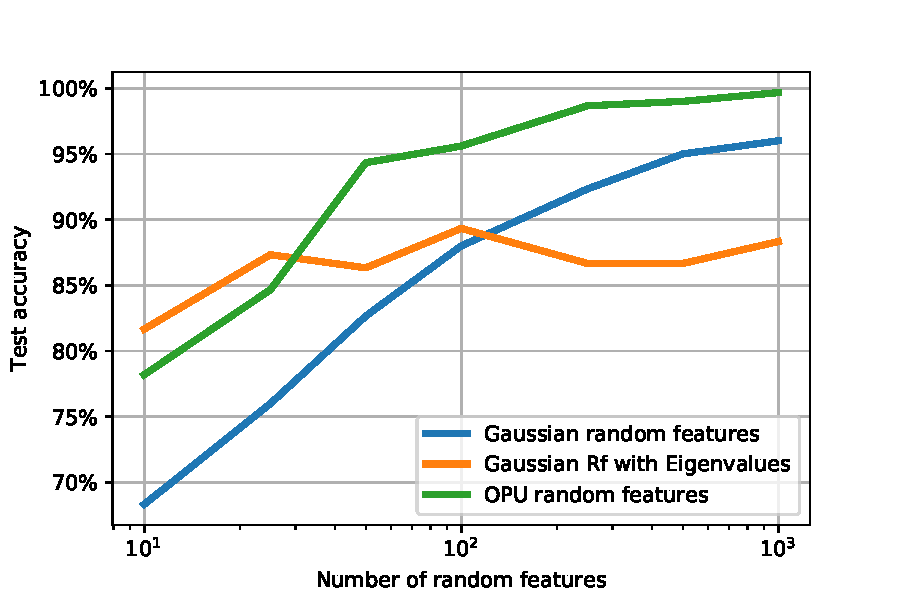
\includegraphics[width=4.0cm]{figs/phi_comparison(1).pdf}}
%  \vspace{1.5cm}
  \centerline{(a) RF maps}\medskip
  \label{subfig:RF_maps}
\end{minipage}
\hfill
\begin{minipage}[b]{0.48\linewidth}
  \centering
  \centerline{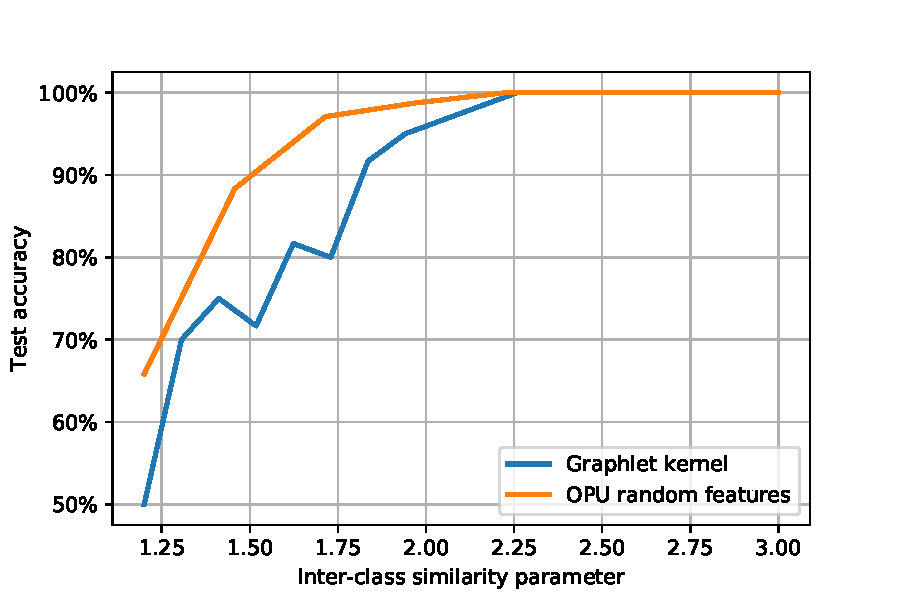
\includegraphics[width=4.0cm]{figs/gk_vs_opu.pdf}}
%  \vspace{1.5cm}
  \centerline{(b) $\varphi_{OPU}$ Vs. $\match$}\medskip
\end{minipage}
%
\begin{minipage}[b]{1.0\linewidth}
  \centering
  \centerline{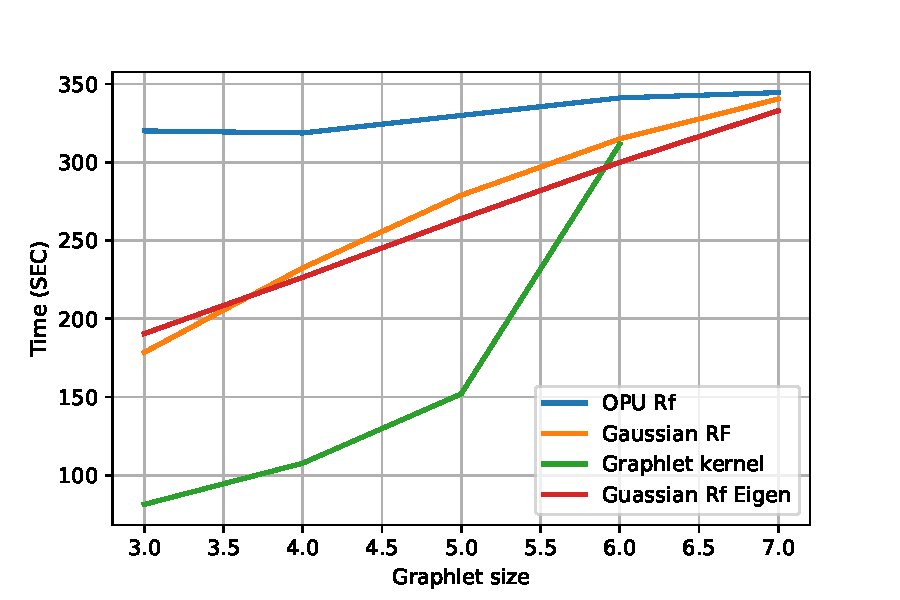
\includegraphics[width=6cm,height=3.6cm]{figs/computational_comp.pdf}}
%  \vspace{2.0cm}
  \centerline{(c) Computation cost}\medskip
\end{minipage}
\caption{Comparing different $\varphi$ maps in $GSA-\varphi$. (a) test accuracy when using RF maps with $k=6$ while varying $m$. (b) test accuracy of $GSA-\varphi_{OPU}$ and $GSA-\match$  fixing $k=5$ while varying $r$. (c) Computation time as a function of $k$. If not specified:  $r=1.1$, $s=2000$, $m=5000$ and $\sigma=0.1$.}
\label{fig:diff_phi}
%
\end{figure}

\subsection{Comparing $GSA-\varphi_{OPU}$ against GIN model}\label{sec:vs_GIN}

Fig \ref{fig:GCN} provides a comparison in test accuracies between $GSA-\varphi_{OPU}$ and  GIN-based GCN model when varying the problem difficulty $r$. We observe that for graphlet sizes $>5$, both RW and uniform sampling perform similarly well in $GSA-\varphi_{OPU}$. And since RW sampling, as expected, provide more consistent results when the graphlet size $k$ varies, it is considered in this comparison.
We see that $GSA-\varphi_{OPU}$ with RW  performs better when the graphlet size is greater than 4. We note that we do not report the computational time for GIN, since it is highly dependent on high-speed graphical processing units (GPUs) to do the training process.

\begin{figure}[htb]
%
\begin{minipage}[b]{.48\linewidth}
  \centering
  \centerline{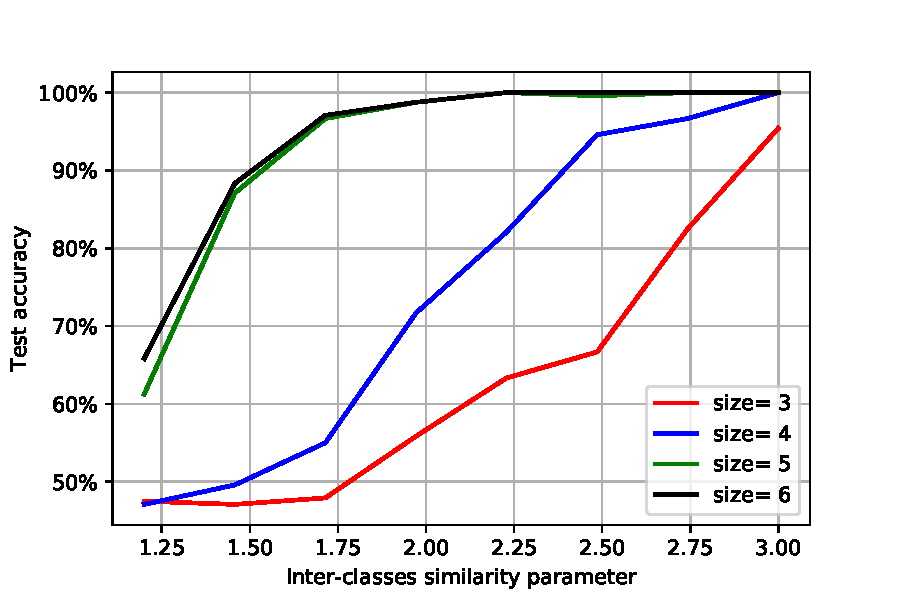
\includegraphics[width=4.0cm]{figs/LightOn_adj_SBM_Similarity_graphlet_size.pdf}}
%  \vspace{1.5cm}
  \centerline{(a) $\varphi_{OPU}$\& uniform sampling}\medskip
\end{minipage}
\hfill
\begin{minipage}[b]{0.48\linewidth}
  \centering
  \centerline{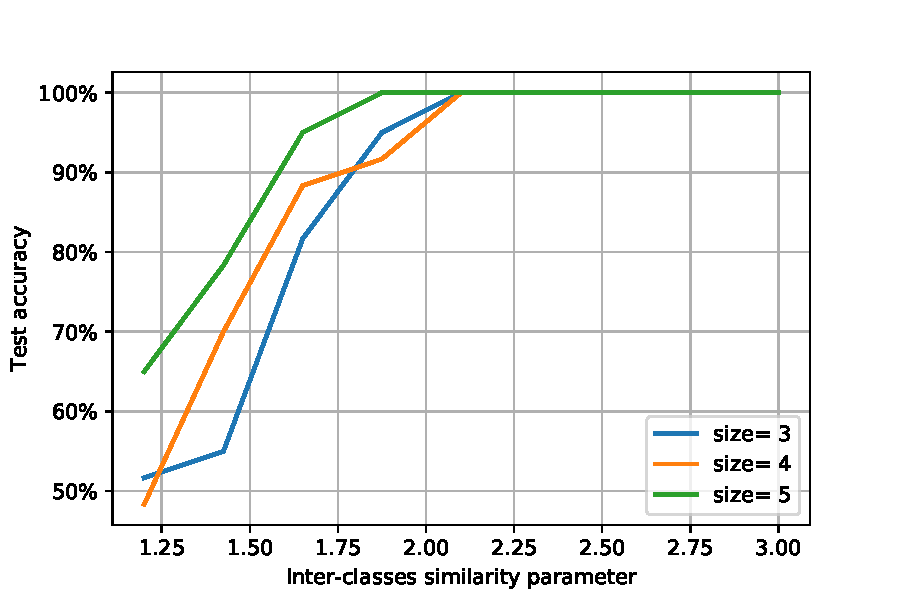
\includegraphics[width=4.0cm]{figs/LightOn_adj_SBM_similarity_graphlet_size_RW.pdf}}
%  \vspace{1.5cm}
  \centerline{(b) $\varphi_{OPU}$\& RW sampling}\medskip
\end{minipage}
%
\begin{minipage}[b]{1.0\linewidth}
  \centering
  \centerline{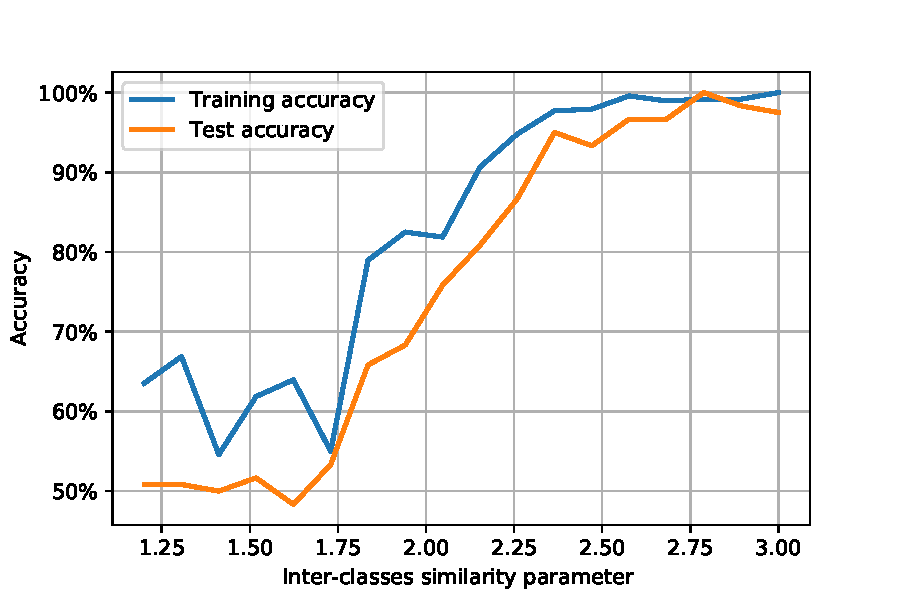
\includegraphics[width=6cm,height=3.6cm]{figs/GCN.pdf}}
%  \vspace{2.0cm}
  \centerline{(c) GIN-based GCN model}\medskip
\end{minipage}
\caption{Comparing test accuracies of $GSA-\varphi_{OPU}$ and GIN-based GCN network when varying the problem difficulty $r$. We used $GSA-\varphi_{OPU}$ with uniform sampling in (a) and with random walk sampling in (b). In both cases: $s=2000$ and $m=5000$. (c) The model consists of 5 GIN layers then two fully connected layers, the dimensions of hidden layers  equal 4.}
\label{fig:GCN}
%
\end{figure}


\subsection{$GSA-\varphi_{OPU}$ on D\&D dataset}
\begin{figure}[htb]
\begin{minipage}[b]{1.0\linewidth}
  \centering
  \centerline{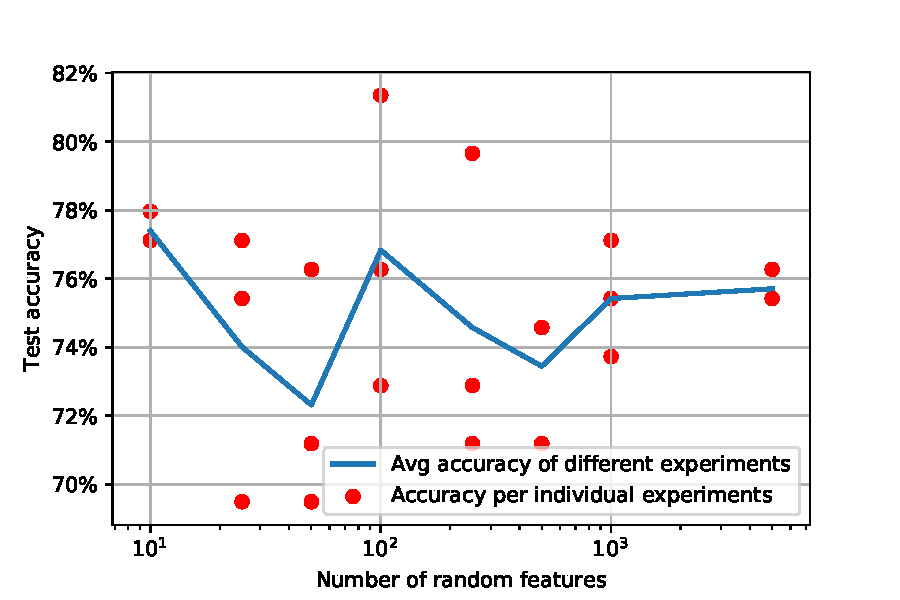
\includegraphics[width=6cm,height=3.6cm]{figs/DD.pdf}}
%  \vspace{2.0cm}
\end{minipage}
\caption{$GSA-\varphi_{OPU}$ test accuracy on D\&D. With  $k=7$, $s=4000$. Varying the value of $m$, the experiment is done five times, then the $5$ resulted accuracies are averaged.}
\label{fig:DD}
%
\end{figure}
In Fig \ref{fig:DD}, we have the the test accuracy with varying value of $m$ and fixed $s=4000 , k=7$. Where for each value of $m$ we conduct the experiment 5 times and take the average accuracy. Although we do not observe a clear, steady average improvement in accuracy when $m$ grows, the results of the 5 corresponding experiments get more concentrated around the average value, giving a desirable reduced variance between experiments. On the other hand, at low $m$ accuracy results show high variance between experiments, which might be accentuated by the fact that nodes features are ignored. However, using node features is without doubt necessary to reach state-of-the-art results, and it is an open question how to incorporate that in our algorithm, but our goal here is mainly to test our algorithm on real data as a proof of concept.


% To start a new column (but not a new page) and help balance the last-page
% column length use \vfill\pagebreak.
% -------------------------------------------------------------------------
%\vfill
%\pagebreak

\section{Conclusion}
\label{sec:Conclusion}
In this work, we proposed a family of algorithms that combines graph sampling with efficient mappings instead of graphlet matching, which requires an expensive isomorphism test. Then, we proposed to choose this mapping as kernel random features, and showed a concentration of the random embedding around the MMD metric. Finally, while classical random features still require expensive matrix-vector multiplication, we used optical random features projections, which can be computed in constant time by a recently developed optical hardware, to get the algorithm's fastest version. Our Experiments showed that it is significantly faster than traditional graphlet kernel and generally performs better while concentrating around a well-defined MMD metric. Furthermore, in our settings it even performed better than a particular graph convolutional networks on graph classification.

 A major point left open to be analyzed is how to use our algorithm to classify graphs with node features. It is known that graph convolutional networks (GCN) have limits in learning just from the graph structure. So, one promising possibility is to use our algorithm to generate features embeddings on the graph level, and then feed these embeddings with the nodes' features of the graph to a deep neural network. Doing this, we take advantage of the speed of both our algorithm and GPUs. On the theoretical side, the properties of our new MMD metric could be further analyzed on particular models of graphs to get a concentration with higher certainty. 


\vfill\pagebreak

% References should be produced using the bibtex program from suitable
% BiBTeX files (here: strings, refs, manuals). The IEEEbib.bst bibliography
% style file from IEEE produces unsorted bibliography list.
% -------------------------------------------------------------------------
\bibliographystyle{IEEEbib}
\bibliography{strings,refs}

\end{document}
